\documentclass[tikz]{standalone}
\usepackage{amsmath}
\usepackage{amssymb}
\usepackage{amsfonts}
\usepackage{tikz}

\thispagestyle{empty}
\begin{document}

	
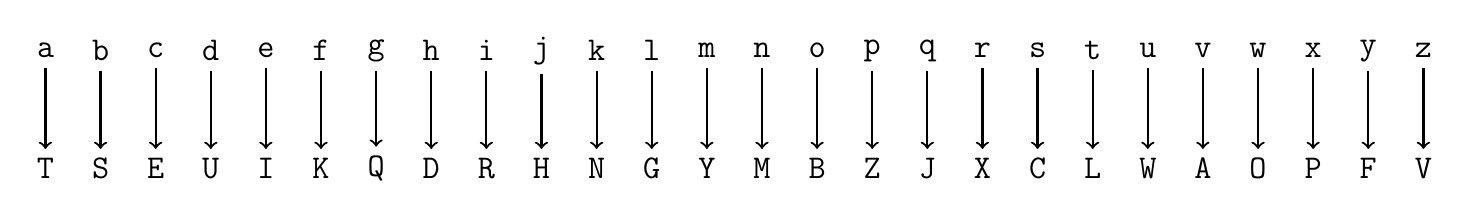
\begin{tikzpicture}[every node/.style={font=\ttfamily\large}, x=0.7cm, y=1.5cm]

% Set the shift amount
\def\shift{3}

% Plaintext row (lowercase)
\foreach \i in {0,...,25} {
	\node (p\i) at (\i, 1) {\char\numexpr`a+\i\relax};
}

\node (c0) at (0,0) {T};
\node (c1) at (1,0) {S};
\node (c2) at (2,0) {E};
\node (c3) at (3,0) {U};
\node (c4) at (4,0) {I};
\node (c5) at (5,0) {K};
\node (c6) at (6,0) {Q};
\node (c7) at (7,0) {D};
\node (c8) at (8,0) {R};
\node (c9) at (9,0) {H};
\node (c10) at (10,0) {N};
\node (c11) at (11,0) {G};
\node (c12) at (12,0) {Y};
\node (c13) at (13,0) {M};
\node (c14) at (14,0) {B};
\node (c15) at (15,0) {Z};
\node (c16) at (16,0) {J};
\node (c17) at (17,0) {X};
\node (c18) at (18,0) {C};
\node (c19) at (19,0) {L};
\node (c20) at (20,0) {W};
\node (c21) at (21,0) {A};
\node (c22) at (22,0) {O};
\node (c23) at (23,0) {P};
\node (c24) at (24,0) {F};
\node (c25) at (25,0) {V};

% Arrows from plaintext to ciphertext
\foreach \i in {0,...,25} {
	\draw[->, thick] (p\i) -- (c\i);
}

\end{tikzpicture}

\end{document}
